\chapter{Relational data}
\label{sect:relational}
Much of the well-structured data used in statistical organizations is stored in
the form of \emph{records}, more formally called \emph{relations}. This Chapter
gives a brief introduction to classical relational database theory.


\section{Relations}
The basic concept underlying classical databases is the idea of a combination
of values, called a \emph{tuple} that are related to one another. The relation
between the values consists of the fact that they are pertain to the same
entity. As an example consider the following tuple.
\begin{equation}
(Id=1, Name="Alice", Age=7, Owns=\{puzzle, bicycle\}).
\label{eq:alice}
\end{equation}
This tuple describes several attributes of a real-world person.  In this case,
the tuple holds the name of a 7 year old person called Alice, who owns a
bicycle and a puzzle.
\begin{terminology}{Tuple}
A \emph{tuple} is a combination of values $(x_1, x_2,\ldots, x_p)$ that take
values in predefined domains.
\end{terminology}
We have introduced a bit of terminology here that needs to be made more precise
for the coming discussion. First of all, we introduced the term \emph{entity}.
An entity is a particular object or event in the real world.  An example of a
real-world entity is \emph{Willem-Alexander Claus George Ferdinand, King of the
Netherlands, Prince of Oranje-Nassau, Squire of Amsberg}.  Each entity is of a
certain \emph{entity type}. The entity type describes all entities that that
belong to a certain group. What constitutes an entity type is in practice
largely a matter of choice. For example we could think of the entity type
`people living in the Netherlands', and define it as `any person who is
registered to live in a Dutch municipality'. Under this condition
\emph{Willem-Alexander Claus George Ferdinand, King of the Netherlands, Prince
of Oranje-Nassau, Squire of Amsberg} is indeed of entity type `people living in
the Netherlands`. Sometimes this is also expressed by saying that
\emph{Willem-Alexander Claus George Ferdinand, King of the Netherlands, Prince
of Oranje-Nassau, Squire of Amsberg} is an \emph{instance} of the type `people
living in the Netherlands`.
%
\begin{terminology}{Entity and Entity Type}
An \emph{entity type} defines a population of entities. An entity
is a real-world object or event. If an entity belongs to a certain
entity type, we say that it is an \emph{instance} of this type.
\end{terminology}

Entities are characterised by their properties. In database-language these are
called \emph{attributes} while statisticians call them \emph{variables}.  It is
important to realize that entities of the same type share an attribute set. For
example, every `person living in the Netherlands' has a `municipality of
residence', namely the municipality where they are registered. Some persons
living in the Netherlands may also own a house on a Greek peninsula. But since
this is not true for all persons living in the Netherlands, the attribute `size
of house on Greek peninsula' is not an attribute for this entity type.
\begin{terminology}{Attribute}
An attribute is a property associated with an entity.  If two entities are of
the same type, they have the same set of attributes, possibly with different
attribute values.
\end{terminology}

This example highlights another common principle: entity types are usually
defined by starting with a broad type and then fixing one or more attributes.
For example, we can start with the entity type `person' and fix the attribute
`municipality' to municipality in the Netherlands. There is one other way of
defining an entity type, and that is by simply listing the entities that belong
to the type. For example, one may define the entity type of `All People with
Dutch Nationality in 2017` by giving a list of all Dutch Social Security
numbers that existed in 2017.


\section{Normalization}
A relational database stores collections of similar tuples.  Normal people call
such a collection a Table, but database theorists call this a \emph{Relation}.
\begin{terminology}{Relation}
A \emph{relation} is a set of tuples, where all tuples have attributes in the
same domains, in the same order.
\end{terminology}
For two tuples (normal people call them records) to be in the same relation,
they must have the same number of attributes and those attributes must be of
the same data type. There are generally several ways of distributing the same
information over relations and tuples in a database. For example, the
information about Alice in Equation~\eqref{eq:alice} can also be represented as a set of
tuples, like so.
\begin{equation}
\begin{array}{l}
(Id=1, Name=``Alice'')\\
(Id=1, Age=7)\\
(Id=1, Owns = \{puzzle, bicycle\}).
\end{array}
\end{equation}

The choice of representation depends on the intended purpose, as also discussed
in Section~\ref{sect:faces}. Historically, focus has been on properties that
were important for business administration systems. Exemplary applications that
drove the development of early database theory are financial and logistic
databases where possibly many users can simultaneously add, remove, or update
data.  An example to keep in mind is a company that buys, sells, and stores
goods at multiple locations.  There are tables of product availability and
location, tables of sales and purchases (transactions) and so on. At any given
time, an employee of the sales department must be able to see whether there is
enough in stock for their next order. A widely applied approach to normalizing
databases was presented in a seminal paper by \citet{codd1970relational}. In
this approach, three levels of database normalization are defined which are
still very much in use today.


\subsection{First normal form}
The idea of the first normal form is to make tuples as simple as possible.
Remember that a tuple is a combination of values, coming from predefined domains.
Another way of expressing this, is to say that the data types of the values in
a tuple must be fixed beforehand. In principle, data types can be very
complex. For example a calendar date is specified by a year, month, and day
(and a time zone which we ignore here) . 
\begin{align*}
(Name =\code{"Alice"}, Birthday = (Year=1991,Month=05,Day=13") )
\end{align*}
So here, the value of $Birthday$ is also a tuple. The domain of $Birthday$
consists of all triples in $\mathbb{N}\times\mathbb{N}\times\mathbb{N}$ that
represent a valid calendar date when their elements are interpreted
respectively as year, month and day.  The first normal form is all about making
tuples as simple as possible, by not allowing data types that are composed of
simpler types.
%
\begin{terminology}{First normal form (1NF)}
A relation is said to be in first normal form (1NF) when:
\begin{itemize}
  \item All tuples have values from the same domains, in the same order. 
  \item There are no duplicate tuples in a relation.
\end{itemize}
\end{terminology}
It is worth noting that there is no intrinsic ordering of tuples (records) in a
relation. This means that in general you can not assume records to be sorted in
any particular way in a database except if you explicitly sort them.

Continuing with the example, we can store Alice's birthday as
$$
(Name =\code{"Alice"}, Birthday = \code{"19910513"} )
$$
The main advantage of 1NF is that operations on the level of relations, like
searching, filtering and sorting are easier to reason about compared to the
situation where tuples might contain complex data values.


The definition of 1NF does raise the question of when something is
\emph{atomic}.  In practice this usually means either a string, a predefined
categorical variable, a Boolean, or a number type such as integer or double
precision, or a date/date-time type.

From a mathematical point of view the idea of atomicity is more subtle. A data
type is atomic only under the set of operations that leave it intact (see also
the definition of algebraic closure in Chapter~\ref{sect:faces}). To clarify
this let us discuss an physical example. In chemistry, atoms and molecules (and
some of their ions) form the 'data type' under chemical reactions.  Which ever
chemical reaction you perform, you can never produce a particle that is not
either an atom (ion) or a molecule. So the set of atoms, molecules and their
ions are closed under chemical reactions. If we allow other, non-chemical
operations, like nuclear fission, we can create particles that are not in the
periodic system, like neutrons, or neutrinos. This shows that the meaning of
`atomic' depends on the operations that you allow. 

Similar to the atoms and molecules in chemistry, we could allow operations on
an \code{Integer} type in a database, other than the familiar arithmetic
operations. For example by pulling them apart into separate bytes, or bits
even. The moral of the story is that there is no absolute definition of
atomicity when it comes to \emph{atomic domains}. In practice, the atomic types
are the simplest data types offered by a programming language or database
system.


%%%%%%%%%%%%%%%%%%%%%%%%%%%%%%%%%%%%%%%%%%%%%%%%%%%%%%%%%%%%%%%%%%%%%%%%%%%%%%%
\subsection{Second normal form}
The intuition behind second normal form, or 2NF in short, is to reduce the
amount of redundancy in storing information and to guarantee a certain
simplicity for each relation. The explicit definition sounds a bit more formal and
requires some explanation.
\begin{terminology}{Second normal form (2NF)}
A relation is said to be in second normal form (2NF) when 
\begin{itemize}
\item it is in 1NF
\item it has no partial dependencies.
\end{itemize}
\end{terminology}
To understand this definition, we need to understand what \emph{partial
dependencies} are. To do so, suppose we have a database with the following
relations.
\begin{center}
\begin{tabular}{|cccc|}
\multicolumn{4}{l}{Ownership}\\
\hline
PersonId & ProductId  & Nr & Shop           \\
\hline
1  &   107   &2  & Toy store \\
1  &   101   &1  & Bicycle store\\
2  &   104   &1  & Toy store\\
\hline
\end{tabular}
$\:\:$\begin{tabular}{|cc|}
\multicolumn{2}{l}{Products}\\
\hline
Id  & Product \\ 
\hline
101 & bicycle\\
104 & ball   \\
107 & puzzle \\
\hline
\end{tabular}$\:\:$\begin{tabular}{|ccc|}
\multicolumn{2}{l}{Persons}\\
\hline
Id  & Name & Age \\ 
\hline
1 & Alice & 7\\
2 & Bob   & 6\\
\hline
\end{tabular}
\end{center}
In the first relation, the key `PersonId' identifies a person whose properties are
stored in the third relation, while the key `ProductId' identifies an object in the
second relation. Together, these two keys completely identify how many objects
of a given type each person owns. For example, we can ask: `how many puzzles
does Alice own?' and look up that information by finding the key combination
$(\textrm{Id}=1, \textrm{Object}=107)$ in the relation `Ownership'.  Compare this
with the situation for the `Shop' attribute. The value of `Shop' does not
depend on `PersonId` and `ProductId`, but only on `ProductId`. One could say that it is
over-identified, or in data-base terminology it only \emph{partially depends}
on the keys available in the relation.  We can improve this situation by moving
the `Shop` variable to the `Products' relation.
\begin{center}
\begin{tabular}{|ccc|}
\multicolumn{3}{l}{Ownership}\\
\hline
PersonId & ProductId  & Nr   \\
\hline             
1  &   107   &20     \\
1  &   101   &5     \\
2  &   104   &3     \\
\hline
\end{tabular}$\textrm{ }$\begin{tabular}{|ccc|}
\multicolumn{3}{l}{Products}\\
\hline
Id  & Product & Shop          \\ 
\hline                       
101 & bicycle& Bicycle store     \\
104 & ball   & Toy store \\
107 & puzzle & Toy store     \\
\hline
\end{tabular}$\textrm{ }$

\begin{tabular}{|ccc|}
\multicolumn{2}{l}{Persons}\\
\hline
Id  & Name & Age \\ 
\hline
1 & Alice & 7\\
2 & Bob   & 6\\
\hline
\end{tabular}
\end{center}
Now none of the relations have attributes with partial dependencies, which
brings them in second normal form. Of course, we do see that there is some
redundancy in data storage since we have some duplicates for the `Shop`
variable. This will be remedied in the third normal form. But before we get to
that, we need to discuss something about keys.

As you may have noticed, we silently introduced the term `key' into the
discussion.  In real-world databases, each and every tuple (record) is uniquely
identified by an explicitly defined key or combination of keys. Such a key is
usually an otherwise meaningless number that carries no information except the
identity of the entity that is described by the tuple. Examples include social
security and passport document number. When a single key identifies each tuple,
this is called the \emph{primary key}. If no such key is provided by the
database designer, database software will typically create one in the
background, possibly invisible to the user. In formal database theory however,
there is no concept of key as a special kind of attribute. In formal theory one
works with sub-tuples, called \emph{candidate keys} that uniquely identify the
other values in the tuple. For a given relation, there may be multiple
candidate keys, with different numbers of attributes in them. This level of
abstraction makes database theory more general but also more cumbersome to
discuss, which is why they we do not discuss it here.


%%%%%%%%%%%%%%%%%%%%%%%%%%%%%%%%%%%%%%%%%%%%%%%%%%%%%%%%%%%%%%%%%%%%%%%%%%%%%%%
\subsection{Third normal form}
The intuition behind the third normal form is again fairly easy to state.  To
avoid duplication of information, store tuples that represent different entity
types in different relations. Continuing with the example of the previous
paragraph, we see that in the second relation, values of the attribute `Shop'
are duplicated in the second relation. Now suppose we want to change 'Toy
store' into `Department store'. For data in this form we need to update two
fields in the second relation. We can solve this by creating a fourth relation
with different `Shops'.  The result is a set of relations that are interlinked
by shared keys, without data duplication.
%
\begin{center}
\begin{tabular}{|ccc|}
\multicolumn{3}{l}{Ownership}\\
\hline
PersonId & ProductId  & Nr   \\
\hline             
1  &   107   &20     \\
1  &   101   &5     \\
2  &   104   &3     \\
\hline
\end{tabular}
$\textrm{ }$\begin{tabular}{|ccc|}
\multicolumn{3}{l}{Products}\\
\hline
Id  & ProductId & ShopId         \\ 
\hline                       
101 & bicycle& S2     \\
104 & ball   & S1 \\
107 & puzzle & S1     \\
\hline
\end{tabular}$\textrm{ }$\begin{tabular}{|ccc|}
\multicolumn{3}{l}{Persons}\\
\hline
Id  & Name & Age \\ 
\hline
1 & Alice & 7\\
2 & Bob   & 6\\
\hline
\end{tabular}$\:\:$\begin{tabular}{|cc|}
\multicolumn{2}{l}{Shops}\\
\hline
Id  & Shop   \\ 
\hline
S1 & Toy Store \\
S2 & Bicycle Store\\
\hline
\end{tabular}
\end{center}
Now, if we update the label `Toy store' to `Department store' it only needs to
be done in a single attribute of a single tuple in a single relation, and all
queries on this set of relations done afterwards must return the new label.


We are now ready to move on to the formal definition of the third normal form.
\begin{terminology}{Third normal form (3NF)}
A relation is said to be in third normal form when
\begin{itemize}
\item it is in 2NF
\item there are no non-prime attributes that are transitively dependent on a key.
\end{itemize}
\end{terminology}
A non-prime attribute is an attribute that is not a key or part of a set of
attributes that together form a key (that is, a set of attributes that uniquely
identify each record). This non-primality condition is really just theoretical
fine-print. It is necessary to define 3NF without explicitly assuming that one
of the attributes in a relation is an identifying variable.  In databases we
always do have such a variable, so we'll use that in the example. The key
concept in the definition is \emph{transitive dependency}.  We have seen what a
dependency is: the value of variable $X$ determines what the value of variable
$Y$ must be. We can denote this with $X\to Y$. For example in the the following
table we have $\textrm{Id}\to \textrm{Object}$.
\begin{center}
\begin{tabular}{|ccrc|}
\multicolumn{4}{l}{Products}\\
\hline
Id  & Product & Price &Shop          \\ 
\hline                       
101 & bicycle& 250,00 &Bicycle store     \\
104 & ball   & 3,50   &Toy store \\
107 & puzzle & 5,00   &Toy store     \\
\hline
\end{tabular}
\end{center}
Such a dependency is called a \emph{functional dependency}. To be precise, the
notation $X\to Y$ means that `whenever two tuples have the same value for
$X$, they have the same value for $Y$. It follows that if we have $X\to Y$ and
we have $Y\to Z$ then this must imply $X\to Z$. This is called the
\emph{transitive property} of functional dependencies.

Now let's take a look at the above table. We have $\textrm{Id}\to
\textrm{Product}$, but we also have $\textrm{Product}\to\textrm{Shop}$.
Namely, for any two Objects that are the same, we have the same Shop (observe
that the converse is not true). This is
trivial here, since every `Product' occurs only once, but nevertheless we see
that
$$
\textrm{Id}\to\textrm{Product}\textrm{ and }\textrm{Object}\to\textrm{Shop}
$$
and therefore we must have the transitive dependency
$$
\textrm{Id}\to \textrm{Shop}.
$$
In other words, the shop type depends indirectly on the identifying key for
`Product'. 

Bringing a relation into third normal form amounts to bringing it first into
second normal form, and then identify the attribute or attributes that show
transitive dependence on other (sets of) attributes. The transitively dependent
attributes are then moved to a separate table.


Any database can in principle be automatically put into 3NF, although in
general there may be more than one solution and some steering based on domain
knowledge is likely to be necessary.  For example, we see in the example
that `Price' also transitively depends on `Id' even though in reality it
is an attribute of a `Product'. In practice, databases are designed by
information analysts and database administrators to be in third normal form in
the first place.  And this brings us to the topic of the next section. 



%%%%%%%%%%%%%%%%%%%%%%%%%%%%%%%%%%%%%%%%%%%%%%%%%%%%%%%%%%%%%%%%%%%%%%%%%%%%%%%
\section{Entity-Relationship diagrams}
\label{sect:erd}
The basic recipe for designing a particular database structure sounds deceivingly
simple:
\begin{enumerate}
\item Identify all the entity types and their properties.
\item Create relations with tuples of the form
$$
(Id, Property_1, Property_2,\ldots,Property_n),
$$
where $Id$ is a \emph{primary key}.
\item A connection between two entities of different entity types is
represented as a relation that contains the primary keys of both entities.
\end{enumerate}

In practical situations, the number of entity types can grow quickly.  Consider
again as an example the situation of Alice and Bob, who own a few objects, that
were bought in a few stores. We've seen that in 3NF there are three obvious
entity types involved, namely `Person' (Alice and Bob), `Object' (bicycle,
ball, puzzle), and `Shop'. Moreover there is an entity type that expresses an
`Ownership' relation between `Person' and `Object'. This is an entity type
because it has unique properties that can not be attributed to a person or
object alone. Here it is only the Size of the ownership (`Nr'), but we can also
think of a starting and ending time of ownership as relevant attributes of this
relation.

Because relations and their interconnections tend to quickly gain complexity,
their design is usually represented graphically in something called an
\emph{entity-relationship diagram} (ERD). As an example, consider the ERD of
the Alice and Bob example in Figure~\ref{fig:erd}.
\begin{figure}[h]
\centering
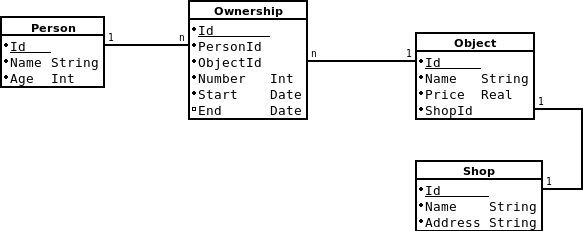
\includegraphics[width=\textwidth]{fig/alice_bob.png}
\caption{Entity-Relationship diagram of people owning objects
bought in shops for a certain price.}
\label{fig:erd}
\end{figure} 
In this diagram, each entity type and its properties are represented in a box.
In this case we also added the type of each property, and labeled the unique
identifier with an asterisk. Whenever the unique identifier (\emph{primary
key}) of one entity occurs in the table of another entity, this is called a
\emph{foreign key}.  This is indicated with a line between boxes that connects
the primary key of one relation with the foreign key in another relation. The
lines are labeled with the type of relationship. For example, the `Id' of a
Person can occur multiple ($n$) times as a foreign key in the `Ownership'
relation.  Whether a connection between two relations is one-to-one,
one-to-many, or many-to-many is called the \emph{arity} of the connection.
%
\begin{terminology}{Primary key, foreign key}
A primary key is a code that uniquely identifies an entity in the relation
representing that entity type. A foreign key is an identifier of one entity
type that occurs in the relation representing another entity type.
\end{terminology}
%
The entity-relationship diagram shown in Figure~\ref{fig:erd} graphically
represents a simple \emph{database schema}. A database schema is a formal
representation of the structure of a database, this includes choices such as
which relations are there, what data is allowed to enter those relations (and
what not) and what are the interconnections between the relations. There are
many tools available that allow one to specify a schema graphically, as in
Figure~\ref{fig:erd}. The software then creates a formal specification for a
particular database management system (DBMS).
\begin{terminology}{Database schema}
A database schema denotes, in a formal (programming) language the
structure of a database.
\end{terminology}

Over time, many variations of entity-relationship diagrams have been developed.
They differ for example in the way the \emph{arity} of connections are
represented.  In some styles an entity type must always be a noun, while a
relation must always be a verb.  In this paragraph we only highlight the most
important bits, as we will return to more formal information modeling in
Chapter~\ref{sect:uml}. The elements we have discussed here are enough to give
a rough sketch for databases


%%%%%%%%%%%%%%%%%%%%%%%%%%%%%%%%%%%%%%%%%%%%%%%%%%%%%%%%%%%%%%%%%%%%%%%%%%%%%%%
\section{Introduction to relational algebra}
Relational algebra consists of a set of basic operations that combine or alter
relations (sets of similar tuples). The basic operations are very general, and
do not depend on type of database, programming language used, or other
implementation details. In fact there are many implementations of these basic
ideas, an we will discuss two of them at the end of this Section.

But before continuing it is worth spending a few words on why having an
`algebra' is important. Recall that the important property of being algebraic
is to have operations that turn things into other things of the same type. Let
us illustrate this with a little algebra we all know. Consider the following
exercise.
$$
\frac{3\cdot 2 + 3\cdot5}{7}
$$
There are several ways to compute the result. The most straightforward way
is the following.
\begin{enumerate}
\item Compute $3\cdot 2=6$, and store the result as $x$.
\item Compute $3\cdot 5=15$, and store the result as $y$.
\item Compute $x+y=6+15=21$, and store the result as $z$.
\item Compute $z/7=21/7=3$.
\end{enumerate}
In total we have done three additions and one division. However, since we know
the rules of arithmetic we can do things more efficiently as follows.
\begin{enumerate}
\item Rewrite the exercise as
$
{3\cdot(2+5)}/{7}
$
\item Compute $2+5$ and rewrite by substituting the answer. We are left with
$
{3\cdot 7}/{7}
$
\item cross out the 7 in the denominator against the 7 in the numerator,
and we are done.
\end{enumerate}
Here, we only needed to evaluate a single calculation (adding 2 and 5)
explicitly. Thus, by using algebraic properties of addition, multiplication and
division we were able to save on the number of calculations, at the cost of
some rewriting. 

Having an algebra of operations, together with strict rules about their like
execution order, allows one to simplify calculations significantly.  For a
simple calculation as just shown, rewriting may actually take more time than a
straightforward calculation. But when the objects of calculation are possibly
large relations with data rather than a few numbers, this balance is likely to
tilt the other way.  Indeed, database systems will typically optimize
user-defined operations on data by shuffling their order to minimize execution
time, memory usage, or a combination of both.

\subsection{Basic operations}
The basic operations on relations are usually divided into set operations
(remember that a relation is a set of tuples) unary operations, and binary
operations (joins).  The fact that tables are sets is important insofar that it
implies that the relations can not be expected to be ordered in any way. So as
far as relational algebra is concerned, the tables
$$
\begin{array}{|ll|}
\hline
Name & Height\\
\hline
Mary & 167\\
Eddy & 180\\
John & 178\\
\hline
\end{array}
\textrm{ and }
\begin{array}{|ll|}
\hline
Name & Height\\
\hline
John & 178\\
Eddy & 180\\
Mary & 167\\
\hline
\end{array}
$$
are exactly the same. In fact, the tabular representations above should be considered
just as a convenience. In principle we are working with a set of ordered tuples, for
which the standard mathematical notation is
$$
\{(John, 178), (Eddy,180), (Mary, 167)\}.
$$

There are three binary set operations that work on relations with the same
attributes: set Union $A\cup B$, set Difference $A-B$, and set Intersection
$A\cap B$. Below are examples of each operation.

Union (only works for relations with the same attributes).
$$
\begin{array}{|ll|}
\hline
Name & Height\\
\hline
Eddy & 180\\
\hline
\end{array}
\cup
\begin{array}{|ll|}
\hline
Name & Height\\
\hline
Mary & 167\\
John & 178\\
\hline
\end{array}
=
\begin{array}{|ll|}
\hline
Name & Height\\
\hline
Eddy & 180\\
Mary & 167\\
John & 178\\
\hline
\end{array}
$$
Difference (only works for relations with the same attributes).
$$
\begin{array}{|ll|}
\hline
Name & Height\\
\hline
Eddy & 180\\
Mary & 167\\
John & 178\\
\hline
\end{array} 
-
\begin{array}{|ll|}
\hline
Name & Height\\
\hline
Eddy & 180\\
John & 178\\
\hline
\end{array} 
=
\begin{array}{|ll|}
\hline
Name & Height\\
\hline
Mary & 167\\
\hline
\end{array}
$$
Intersection (only works for relations with the same attributes).
$$
\begin{array}{|ll|}
\hline
Name & Height\\
\hline
Eddy & 180\\
Mary & 167\\
John & 178\\
\hline
\end{array} 
\cap
\begin{array}{|ll|}
\hline
Name & Height\\
\hline
Eddy  & 180\\
John  & 178\\
Alice & 192\\
\hline
\end{array}
=
\begin{array}{|ll|}
\hline
Name & Height\\
\hline
Eddy  & 180\\
John  & 178\\
\hline
\end{array}
$$
In principle one of these `basic relations' is redundant since we can write
intersection as a combination of union and difference (see
Exercise~\ref{ex:settheory}). Having these three basic operations is thus more
a matter of convenience than of theoretical minimalism.



Unary operations are operations that act on a single relation. There are three
unary operations: Projection, Selection, and Rename.  The Projection operation
selects zero or more columns from a relation, returning a possibly smaller relation.
It is denoted as $\Pi_{a_1,\ldots,a_p}$ where the subscripts denote what
columns to select. Here's an example.
$$
\Pi_{Name}\;
\begin{array}{|ll|}
\hline
Name & Height\\
\hline
Mary & 167\\
Eddy & 180\\
John & 178\\
\hline
\end{array}
= 
\begin{array}{|l|}
\hline
Name \\
\hline
Mary \\
Eddy \\
John \\
\hline
\end{array}.
$$
The second unary operation is called Selection. It is denoted $\sigma_\phi$, where
$\phi$ is a Boolean proposition (a selection rule) stating a condition on attributes
in the relation.
$$
\sigma_{Height\leq 170}\;
\begin{array}{|ll|}
\hline
Name & Height\\
\hline
Mary & 167\\
Eddy & 180\\
John & 178\\
\hline
\end{array}
=
\begin{array}{|ll|}
\hline
Name & Height\\
\hline
Mary & 167\\
\hline
\end{array}
$$
The last unary operation is called Rename. It is denoted ${\rho_{a/b}}$ where
$a$ is the name of the attribute to be renamed, and $b$ is the new name.
$$
\rho_{Name/FirstName}\;
\begin{array}{|ll|}
\hline
Name & Height\\
\hline
Mary & 167\\
Eddy & 180\\
John & 178\\
\hline
\end{array}
=
\begin{array}{|ll|}
\hline
FirstName & Height\\
\hline
Mary & 167\\
Eddy & 180\\
John & 178\\
\hline
\end{array}
$$

Finally, there are several types of \emph{join} operations that merge two
relations into a single new relation, based on common values in shared
attributes. The most important one is the \emph{natural join}, denoted
with a `bowtie' symbol: $\bowtie$. This merges two
datasets and only keep the records that can be merged.  This is often referred
to as an \emph{inner join}.
$$
\begin{array}{|ll|}
\hline
Name & Age\\
\hline
John & 25\\
Mary & 34\\
\hline
\end{array}
\;\bowtie\;
\begin{array}{|ll|}
\hline
Name & Height\\
\hline
Mary & 167\\
Eddy & 180\\
John & 178\\
\hline
\end{array}
\;=\;
\begin{array}{|lll|}
\hline
Name & Age & Height\\
\hline
John & 25 & 178\\
Mary & 34 & 167\\
\hline
\end{array}
$$
In formal relational algebra, it is assumed that there are no duplicate keys to
merge on. So for example \emph{Mary} will occurs maximally once in each table
on the left-hand-side (recall the definition of 1NF). In practice duplication
can occur, and we will see in the next section how this is dealt with in
implementations.

The \emph{outer join}, merges two tables on shared attributes with common
values, but also keeps the records that can not be matched. Attributes
of one table that have no match with the other one are left empty.

$$
\begin{array}{|ll|}
\hline
Name & Age\\
\hline
John  & 25\\
Mary  & 34\\
Alice & 57\\
\hline
\end{array}
\;\times\;
\begin{array}{|ll|}
\hline
Name & Height\\
\hline
Mary & 167\\
Eddy & 180\\
John & 178\\
\hline
\end{array}
\;=\;
\begin{array}{|lll|}
\hline
Name & Age & Height\\
\hline
John & 25 & 178 \\
Mary & 34 & 167 \\
Alice& 57 &     \\
Eddy &    & 180 \\
\hline
\end{array}
$$

Both the natural join and the outer join are symmetric, that is $A\bowtie
B=B\times A$ and $A\times B=B\times A$ for any two relations $A$ and $B$. There
are also variants that are \emph{not} symmetric. The \emph{left join}, denoted
$\ltimes$, keeps all records from the left hand side and adds records at the
right hand side where possible. Attributes for records with no match are left
empty.

$$
\begin{array}{|ll|}
\hline
Name & Age\\
\hline
John  & 25\\
Mary  & 34\\
Alice & 57\\
\hline
\end{array}
\;\ltimes\;
\begin{array}{|ll|}
\hline
Name & Height\\
\hline
Mary & 167\\
Eddy & 180\\
John & 178\\
\hline
\end{array}
\;=\;
\begin{array}{|lll|}
\hline
Name & Age & Height\\
\hline
John & 25 & 178 \\
Mary & 34 & 167 \\
Alice& 57 &     \\
\hline
\end{array}
$$
Similarly, there is a \emph{right join} denoted $\rtimes$, that keeps all
records of the right hand side. Finally, there is the \emph{antijoin}
operation, denoted $\triangleright$. The antijoin is not really a join
operation. It selects records from the relation on the left-hand side that can
not be matched with the relation on the right hand side.
$$
\begin{array}{|ll|}
\hline
Name & Age\\
\hline
John  & 25\\
Mary  & 34\\
Alice & 57\\
\hline
\end{array}
\;\triangleright\;
\begin{array}{|ll|}
\hline
Name & Height\\
\hline
Mary & 167\\
Eddy & 180\\
John & 178\\
\hline
\end{array}
\;=\;
\begin{array}{|ll|}
\hline
Name & Age\\
\hline
John  & 25\\
Mary  & 34\\
\hline
\end{array}
$$
Observe that the difference between the antijoin and set intersection is that
for set intersection, we demand that the relation on the left hand side has
the exact same attributes as the relation on the right hand side while
this is not the case for antijoin.

To complete our discussion of relational algebra, we need to define the operator
precedence. That is, just like we agreed that in normal arithmetic, multiplication
comes before addition, we need to define the order of execution when combining
multiple relational operations. The order is defined as follows.
\begin{enumerate}
\item $\sigma$, $\Pi$, $\rho$ (highest precedence ---execute this first when possible)
\item $\bowtie$, $\times$, $\ltimes$,$\rtimes$, $\triangleright$
\item $\cap$
\item $\cup$, $-$.
\end{enumerate}
In this booklet we shall always use brackets to make order of execution
absolutely clear.

\subsection{Implementations}
Relational algebra has been implemented, fully or partially in many tools. Here
we shall briefly discuss two of them: SQL and R package `dplyr'. The latter
tool will be used in the workshop exercise. The goal of this chapter is not to
learn how to work with SQL, but to raise awareness that the formal concepts
introduced so far have real and practical implementations that are used every
day.

The most important implementation of relational algebra is SQL, which stands
for Structured Query Language. SQL is in itself not a tool, but the definition
of a programming language that treats tables as a basic type. This programming
language is implemented in many (commercial) database systems where different
vendors typically create their own dialect of SQL, for example by extending it
with certain capabilities for data analyses. However the basic operations
treated here are usually all present.

Here is an example. Suppose we have a table called `A' and we wish to select the attribute
called `Height'. In SQL this would look something like this.
\begin{verbatim}
  SELECT Height FROM A
\end{verbatim}
So here, \code{SELECT HEIGHT} is a direct translation of $\Pi_{Height}$ and the
whole expression means $\Pi_{Height}A$. If we want to do a left join on the
Name attribute between A and B, and subsequently select `Age' and `Height', we
get the following.
\begin{verbatim}
  SELECT Height, Age FROM 
    A LEFT JOIN B ON Name
\end{verbatim}
Observe that the operator precedence discussed in the previous section ensures
that $A\ltimes B$ is computed first and next `Height' and `Age' are selected.
Readers interested in learning SQL could have a look at the online tutorial
of the W3Schools organization\footnote{
\href{https://www.w3schools.com/sql/default.asp}{https://www.w3schools.com/sql/default.asp}
}.

A second --sort of-- implementation comes with R package `dplyr`.  In R, a
relation is represented by something called a \emph{data.frame}.  There are no
ways to force the absence of duplicates, or even atomicity of its contents, so
this data type is more flexible than the type of relations where relational
algebra was designed for. Although R \citep{Rcore} comes with implementations
of all relational operators that work on data frames, many people find the
syntax implemented in the \code{dplyr} package easier to work with, so this is
what we will discuss here.

To select a column called `Height' from a data frame called `A', in
\code{dplyr} one calls a function called \code{select}.
\begin{verbatim}
  select(A, Height)
\end{verbatim}
Since `dplyr` does not offer a programming language, but a set of functions,
some syntax is needed to take the output of one function and pass it to
the next function. Here we use the so-called pipe operator and work out the
second example.
\begin{verbatim}
  A %>% 
    left_join(B, Name) %>%
    select(Height, Age)
\end{verbatim}
Here, the \code{\%>\%} operator takes the output on the left hand side and
feeds it as the first argument of the functions on the right hand side.  This
is equivalent to storing intermediate results and reusing that in the
calculations.
\begin{verbatim}
  X <- left_join(A, B, Name)
  select(X, Height, Age)
\end{verbatim}
Which syntax is preferred is to an extend a matter of taste. The former syntax
with \code{\%>\%} is quicker to develop, the latter syntax is easier to debug
since intermediate results are available.










\subsection*{Where are we?}
We have see that the concepts of tables and records can be treated formally in
database theory, where they are called respectively relations and tuples.  The
formal treatment yields normalized forms that can be described and designed
graphically using entity-relationship diagrams (database diagrams).  Moreover,
there is a small number of basic operations that can be used to manipulate of
sets of relations. Many commonly used tools implement these operations or
variants thereof so they are ubiquitous in data management.


\newpage
%%%%%%%%%%%%%%%%%%%%%%%%%%%%%%%%%%%%%%%%%%%%%%%%%%%%%%%%%%%%%%%%%%%%%%%%%%%%%%%
\section{Exercises}
\label{sect:exrelational}

\begin{enumerate}
\item Put the following table in 1NF

\begin{tabular}{|cccc|}
\hline
Id & Name  & Age & Owns \\
\hline
1  & Alice & 7 & $\{\textrm{puzzle},\textrm{bicycle}\}$\\
2  & Bob   & 6 & $\{\textrm{ball}\}$\\
\hline
\end{tabular}
\item In official statistics, there are several ways to count businesses. There
are `legal units' which are defined by their registration at the Chamber of
Commerce. There are `Tax' units which are defined as one or more legal units
that together file a tax report.  And then there are `Economic units'. These
are constructed by Official Statisticians by combining one or more legal units
into an establishment that coherently conducts its business. Exemplary cases
are large (multinational) companies that separate activities into different
legal units. It is also possible for multiple legal units to form  a new Tax
unit, but those legal units do not necessarily come from the same economic
unit. How would you store such data? Create a database schema to reflect that.
\item Consider the database schema in Figure~\ref{fig:recordschema} and answer
the following questions.
\begin{enumerate}
  \item How many attributes are there in the employees table?
  \item What are the foreign keys in the `tracks' table?
  \item What is the type of the primary key in `customers'?
\end{enumerate}
\begin{figure}[t]
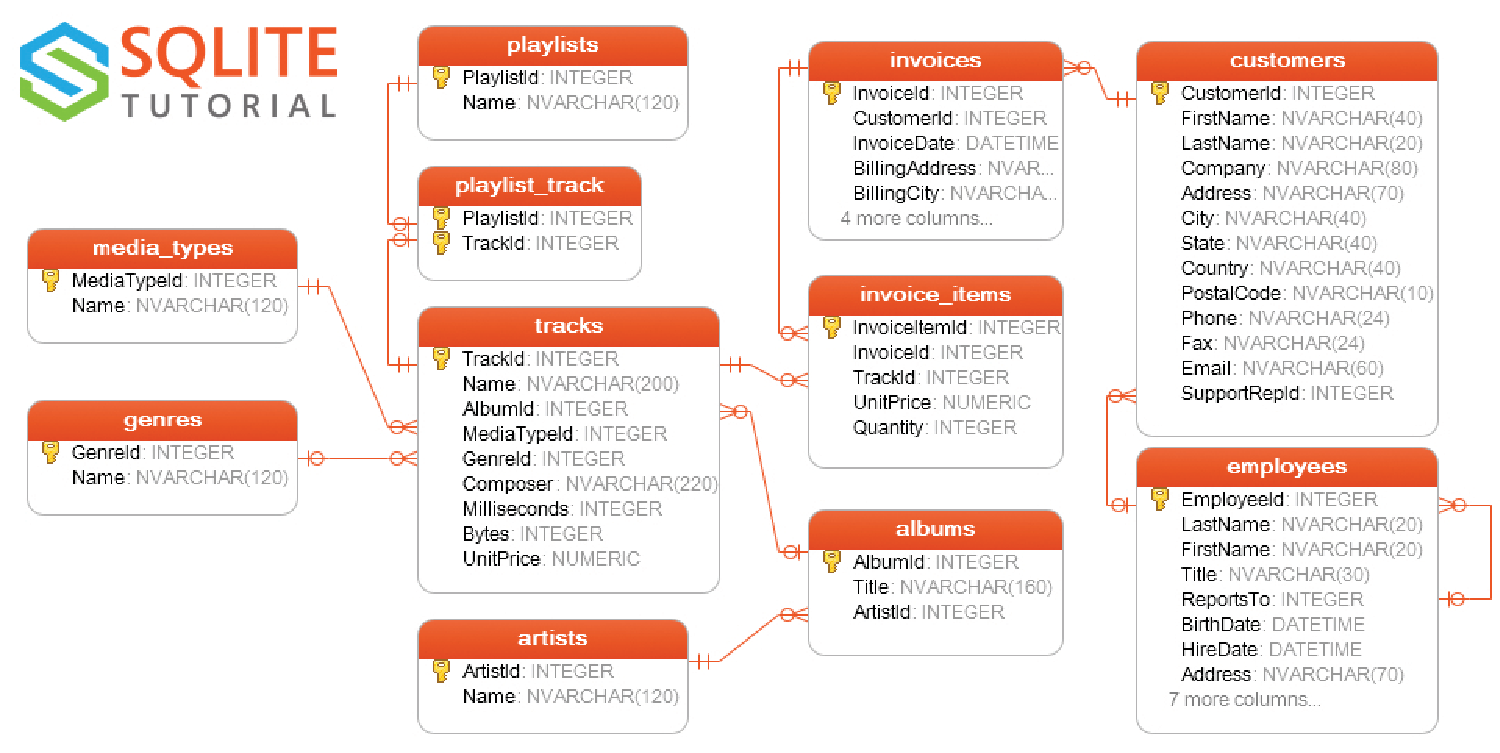
\includegraphics[width=\textwidth]{fig/recordschema.pdf}
\caption{A database scheme for record sales, taken from from the SQLite tutorial 
(\href{sqlitetutorial.net/sqlite-sample-database/}{https://www.sqlitetutorial.net/sqlite-sample-database/}).
}
\label{fig:recordschema}
\end{figure}
\item Create a database schema for the case in Section~\ref{sect:schema}.
\item \label{ex:settheory} Consider the sets $V=\{a,b,c,d,e\}$ and
$W=\{b,d,f\}$.  Show that in this case $V\cap W$ gives the same result as $V\cup W- (V - W)
- (W - V)$. Bonus question: can you prove this is true for any two sets $V$ and $W$?
\item Consider the following two tables.
$$
A =
\begin{array}{|ll|}
\hline
Name & Age\\
\hline
John  & 25\\
Mary  & 34\\
Alice & 57\\
\hline
\end{array}
\;
B = 
\begin{array}{|ll|}
\hline
Name & Height\\
\hline
Mary & 167\\
Eddy & 180\\
John & 178\\
\hline
\end{array}
$$
\label{ex:schema}
Compute the following relations, try to simplify the calculations before
filling in the actual relations.
\begin{enumerate}
  \item $\Pi_{a\in A}(A\ltimes B)$, where $a\in A$ means all attributes occurring in $A$. 
  \item $\sigma_{Age>40} (A\bowtie B)$.
  \item $\sigma_{Age\leq40\land Height\leq 170} (A\times B)$. (The symbol $\land$ means `AND').
  \item $\Pi_{Height}A\bowtie B$.
\end{enumerate}
\item Take a look again at the schema in Figure~\ref{fig:recordschema}. How
would you create the following relations? Use notation from relational algebra
to express this.
\begin{enumerate}
  \item A relation with one tuple for each track, holding Album Title and Track Name.
  \item A relation with Artist, Track, and customerId, so we can identify in what artists
        each customer is interested.
  \item A relation with TrackId and EmployeeId so we can analyze which employee sells most tracks.
\end{enumerate}

\end{enumerate}

\hfill{}Check your answers on page~\pageref{sect:ansrelational}.


\begin{subappendices}
\section{Case: car rentals}
\label{sect:schema}

Your job is to design a database schema for the case below. You can do it on
pen and paper (great to get started!), use a drawing programme, or one of the
many (online) free database schema creators. An example is
\hlink{https://www.dbdesigner.net}{dbdesigner}.  You can use the guest login or
create a free trial account. (Note: you will not be able to save your schema,
but you can export an image or SQL code)\footnote{
This assignment was taken from the Master's Thesis of
\citet{zhang2012suite}.
}.


\subsection*{Part 1}

Our company does car rental business and has several locations with different
address (address consist of street with the number, city, and postal code). In
large cities there can be multiple locations. The cars are classified as
subcompacts, compacts, sedans, or luxury. Each car has a particular model, year
made, and color. Each car has a unique identification number and a unique
license plate.

\subsection*{Part 2}

Cars rented in a particular location may be returned to a different location
(pickup and drop-off). For every car we keep the odometer (km traveled) reading
before it is rented and after it is returned. The car is rented out with full
tank and we record the volume of gas in the tank when the car is returned, but we
only indicate if the tank is empty, quarter full, half full, three quarters
full, or full.

\subsection*{Part 3}

We keep track of which day a car was rented, but not of the time, similarly for
car returning. If a customer requests a specific class (say sedan), we may rent
the customer a higher-class car if we do not have the requested class in the
stock, but we will price it at the level the customer requested (so-called
upgrade). Each car class has its own pricing, but all cars in the same class are
priced the same. 


\subsection*{Part 4}

We have rental policies for 1 day, 1 week, 2 weeks, and 1 month. Thus, if a
customer rents a car for 8 days, it will be priced as 1 week + 1 day. The
drop-off charge only depends on the class of the rented car, the location it was
rented from and the location it is returned to. About our customers, we keep
their names, addresses, possibly all phone numbers, and the number of the
driver’s license (we assume a unique license per person). 

\subsection*{Part 5}

About our employees we keep the same basic information as our customers (we
require that all our employees have a driver’s license). We have several
categories of workers, drivers, cleaners, clerks, and managers. Any of our
employees can rent a car from our company for a 50% discount, if the rental is
less than 2 weeks. However, for any longer rental they must pay 90% of the
regular price. Every employee works in one location only. 

\end{subappendices}


